\documentclass[pdftex,12pt,letter]{article}
\usepackage[binary-units=true]{siunitx}
\usepackage[margin=0.75in]{geometry}
\usepackage{verbatim}
\usepackage{graphicx}
\usepackage{cite}
\usepackage{color}
\usepackage[pdftex,pdfpagelabels,bookmarks,hyperindex,hyperfigures]{hyperref}
\usepackage{xspace}
\usepackage{amssymb}

\usepackage[firstpage]{draftwatermark}


\bibliographystyle{unsrt}

\newcommand{\fixme}[1]{\textbf{FIXME: #1}}    
\newcommand{\pd}{protoDUNE\xspace}

\title{A Proposal for the Single-Phase \pd (NP04) Data Challenges in 2017-2018}
\date{\today}
\author{R.Pordes, M.Potekhin, D. Stefan, R.Sulej}

\begin{document}
\SetWatermarkText{DRAFT}
\SetWatermarkLightness{0.9}
\SetWatermarkScale{3}

\maketitle

\begin{abstract}
\noindent There are two main factors that make it necessary to ensure 100\% readiness of the
end-to-end \pd software and computing complex during the detector commissioning period and
throughout data taking in 2018. First, due to the short run schedule spending any significant amout
of time on debugging will make fulfillment of
the run plan impossible. Second, the Collaboration will need to process and analyze the NP04 data
on a reasonably short time scale (months rather than years) in order to maximize benefits of the
prototype effort for the DUNE R\&D work and CDR cycle, so efficient resource management and
throughput of \pd processing will be of essence right at the beginning of data taking. For these
reasons, and given the \pd schedule,  we propose to conduct two Data Challenges in order to identify
and address potential issues before they can impact the experiment.



\end{abstract}

\tableofcontents

\pagebreak

\section{About this document}
%The Single-Phase \pd experiment (NP04) is characterized by substantial data rates
%and volume, as well as by inherent complexity of its data handlng and processing scheme due
%to properties of its main detector (the Liquid Argon TPC), readout electronics and other factors.
%Initial estimates indicate considerable CPU and storage requirements for production and analysis.
%In order to ensure readiness of the protoDUNE computing infrastructure for data taking
%in 2018, it will be necessary to conduct Data Challenges which are meant to validate
%individual infrastructure and software components, interfaces  as well as the status of overall
%system integration.
The goal of this document is to provide concise information about the proposed \pd Data Challenges
to the infividual working groups in order to coordinate effort and come to a consensus as to the scope,
plans and schedule of the proposed Data Challenges. It does not contain detailed descriptions
and/or designs of the \pd computing
infrastructure elements and the reader is reffered to existing documentation where
needed, with references provided in the text.

\section{The Scope of the Data Challenges}
Information regarding the \pd (NP04) computing is summarized in the \pd-SP Technical Design Report\cite{docdb1794}.
The following components (including infrastructure, middleware and software) can be identified as relevant in the context
of Data Challenges (which will be also referred to as ``DC'' in this document):
\begin{itemize}
\item The DAQ \textbf{Online Buffer} which stores raw data assembled by the Event Builders, as files on disk. The internals
of the DAQ system itself are not within the scope.

\item  \textbf{Beam Instrumentation Interface}. Most of the Beam Instrumentation data is not included into the data stream
handled by the \pd DAQ (whose primary task is to capture data from the TPC and the Photon Detector), and is instead
transmitted to the Beam Instrumentation Database at CERN. It is not available immediately for each triggered event,
and is instead available in batches after each spill cycle of the SPS. Interfacing this system is a task that needs
to be addressed for \pd to be able to validate its beam trigger system.

\item The \textbf{Raw Data Management System}\cite{docdb1212}  which performs data transfers between a few endpoints
at CERN and FNAL starting with the Online Buffer and which is also tasked with proper accounting and handling of Metadata
by interacting with the SAM system at FNAL (see next item). The Data Handling System will inteface the disk-based mass storage
at CERN and FNAL (i.e.\,EOS\cite{eos} and dCache) as well as tape systems (CASTOR and Enstore respectively).
We anticipate using the \textit{Fermi File Transfer System}, also abbreviated as F-FTS\cite{fts} for most of this functionality.

\item The \textbf{Metadata}  -- SAM system at FNAL which comprises the functionality of the file catalog, data storage and
retrieval based on Metadata and can also be used for orchestration of production workflows.

\item \textbf{Data Quality Monitoring} (DQM) which is tasked with running algorithms with turnaround time short enough to provide
actionable results (under and hour) but which won't fit into the computational footprint of the Online Monitoring (a part of DAQ).
To support DQM, the ProtoDUNE Prompt Processing System (\textbf{p3s}) \cite{docdb1811,p3s} has been created and will run any type of\
DQM workload as formulated and programmed by the working groups.

\item \textbf{Calibration and Production Software}. While it is not expected that these components will be finalized
(and some even exist) for at least the first Data
Challenge it is important to have a firm grasp of the required interfaces, data flow patterns and other crucial aspects of
the \pd Production Systems. Having functional prototypes or at least mockups  in place is therefore crucial on the time
scale of the Data Challenges.
An important component of the overall production chain is the \textit{Data Reduction} step along the lines described
in \cite{docdb2089}. In one shape or another it is likely to be included in the production software and will in fact constitute
one of the more CPU-intensive components. Understanding the interfaces and practical implications of this component would
be a useful part of the Data Challenge.

\item \textbf{Analysis Suite Prototypes}. Same comment applies here as to the previous item, i.e.\, while there is no expectation
for the final design and implementation of the analysis chain to exist (especially that it is by nature the most dynamic and
fluid part of all software) it is important to put in place, document and optimize its interfaces with various components
of infrastructure e.g.\,calibration databases, Metadata, software and data provenance controls etc.

\item \textbf{Production Operations Management Service (POMS)}. This service \cite{poms} manages and automates jobs
submission on distributed resources on the Grid. It will be the primary platform for \pd on which to run production and analysis.


\end{itemize}
\noindent Relationship between the various infrastructure and other components listed above is schematically illustrated in
Fig.\ref{fig:dc1}. This diagram relflects the fact that transmission of \pd data is a multistage process and in particular there
will be separate instances of F-FTS transferring the data from the Online Buffer to mass storage at CERN, and then from
CERN to FNAL and elsewhere.

\begin{figure}[tbh]
  \centering
  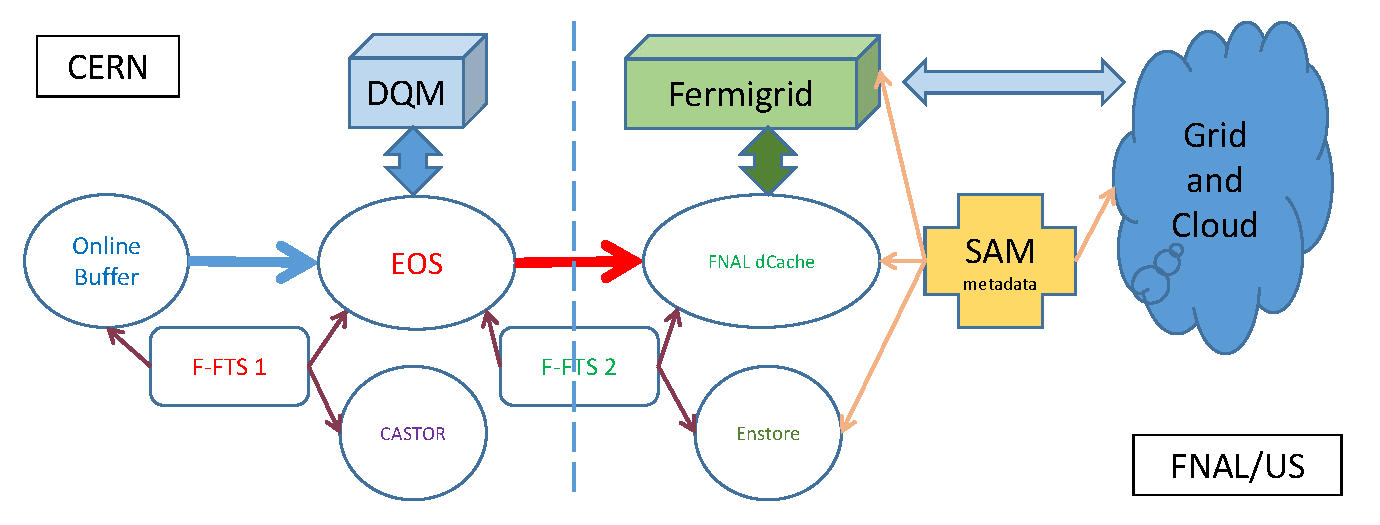
\includegraphics[width=1.0\textwidth]{figures/data_challenge_1.pdf}
  \caption{Schematics of data flow and  processing in \pd data challenges.}
  \label{fig:dc1}
\end{figure}
\noindent Data and production streams which belong to \pd Monte Carlo simulation domain are not included in the
scope of Data Challenges presented here.

\section{Plans for Data Challenges}
\subsection{Work-up to the Data Challenges}
Before any end-to-end data challenge can be meaningul, all individual components and interfaces must undergo
their own functional testing. The following non-inclusive list illustrates the scope of the pre-DC activity:
\begin{itemize}

\item \textbf{Data Transfer and SAM interaction}.  Both F-FTS1 and F-FTS2 components as schematically depicted in Fig.\,\ref{fig:dc1}
must undergo end-to-end functional testing including registration in SAM and sinking data to tape storage both at CERN and FNAL. A test
agent will be created which simulates creation of the raw data files by DAQ, which are written to the Online Buffer and picked up
by the F-FTS for transmission.

\item \textbf{Beam Instrumentation Interface}. At a minimum, mockup schemas for \pd beam detectors must be created in
the CERN Beam Instrumentation Database, and populated with dummy data. An extraction process must be put in place which
``captures'' these data and commits it either to a database managed by \pd or as files on disk (EOS). A prototype or a mockup
of the merging process must be put in place.

\item  \textbf{DQM/p3s}. The prompt processing system must be tested and validated to run with the primary data
staging area being in EOS. The issues of deployment, updating and maintenance of LArSoft and other requisite software
must be resolved.

\item  \textbf{Data Reduction Software}. In one shape or another, data reduction will form a distinct stage in the production chain
in \pd. A prototype of this software module must be tested with simulated data and packaged in a way that is portable across
FNAL and facilities at CERN.

\item  \textbf{Calibration and Production}. This includes running prototypes and mockups of this software utilizing the FNAL POMS.

\item  \textbf{Analysis}. The main point in this exercise to to ready the interface of the analysis software to SAM and other
components of the production system(s). There are no strict requirements to functionality and performance of the analysis
software at this stage.

\end{itemize}
\noindent The work-up period must be completed no later than September 2017. It is expected that Data Reduction, Production, DQM
and othe components will have substantial overlaps and/or commonalities, which must be exploited from the point of view of software
sharing and reuse. One of the goals of the work-up period is to identify such items.

\subsection{Timeline, Reporting and Documentation}
Because of the significant CERN involvement in \pd computing, and to facilitate communication with the CERN IT management
it appears optimal to document the working plans and progress of Data Challenges on the CERN TWiki pages provided by
CENF. More detailed technical documentation regarding components and systems will be managed on DUNE DocDB as before.

The work-up as described above should be completed by September 2017, and reports for each component provided
to the \pd leadership and the \pd-CERN computing liaison representative. DC1 will take place in October 2017.
DC2 will be conducted in February 2018. Each Data Challenge will result in a concise report which will be made available
to the Collaboration and follow-up shall be organized as needed.

\subsection{DC1 Scenario}

\begin{itemize}

\item Simulated raw data is deposited into the Online Bufer by the specially created test agent.

\item The data is detected by F-FTS1 and transmitted to EOS.

\item F-FTS2 initiates data transfer to dCache at FNAL. Contact is made with the Metadata system (SAM) where the files
are registered.

\item Mock-up Beam Instrumentation data is captured by \pd systems and is stored either on a DB server or as files on EOS.

\item Automated process initiates DQM streams in p3s. In DC1, full-blown processing on CERN Tier-0\,\cite{lxbatch}
will not be required and at a minimum the operation of p3s will be validated on the Neutrino Platform cluster\,\cite{neut}.

\item Production team at FNAL submits production jobs using the newly arrived data as input.

\end{itemize}


\subsection{DC2 Scenario}

\begin{itemize}

\item DAQ sends raw data (such as pulser or dummy trigger data) to the Online Bufer.

\item The data is detected by F-FTS1 and transmitted to EOS.

\item F-FTS2 initiates data transfer to dCache at FNAL. Contact is made with the Metadata system (SAM) where the files
are registered.

\item Realistic Beam Instrumentation data is captured by \pd systems and is stored either on a DB server or as files on EOS.

\item Automated process initiates DQM streams in p3s using  CERN Tier-0. At a minimum, ADC and noise spectra (FFT) are produced
and delivered to the user by a Web service.

\item Production team at FNAL submits production jobs using the newly arrived data as input.

\item Analysis chain is activated.

\end{itemize}


\section{Personnel and Responsibilities}

\begin{itemize}

\item Online Buffer and the test agent -- DAQ team

\item Beam Instrumentation Interface -- Beam Instrumentation Group, DB coordinator: J.Paley

\item F-FTS -- FNAL team (lead: A.Norman)

\item p3s -- prompt processing team (lead: M.Potekhin)

\item DQM and production payloads -- DRA team (co-leads: D.Stefan, R.Sulej)

\item Integration consultant -- B.Viren

\item Metadata and SAM -- FNAL SCD (T.Junk, S.Fuess)

\item Analysis -- TBD

\item Coordination -- R.Pordes


\end{itemize}

\clearpage
\begin{thebibliography}{1}

\bibitem{docdb1794}
{DUNE DocDB 1794: \textit{ProtoDUNE-SP Technical Design Report }}\\
\url{http://docs.dunescience.org:8080/cgi-bin/ShowDocument?docid=1794}



\bibitem{docdb1212}
{DUNE DocDB 1212: \textit{Design of the Data Management System for the protoDUNE Experiment}}\\
\url{http://docs.dunescience.org:8080/cgi-bin/ShowDocument?docid=1212}

\bibitem{eos}
{The CERN Exabyte Scale Storage}\\
\url{http://information-technology.web.cern.ch/services/eos-service}


\bibitem{fts}
{The Fermilab File Transfer System}\\
\url{http://cd-docdb.fnal.gov/cgi-bin/RetrieveFile?docid=5412&filename=datamanagement-changeprocedures.pdf&version=1}


\bibitem{docdb1811}
{DUNE DocDB 1811: \textit{Prompt Processing System Requirements for the Single-Phase protoDUNE}}\\
\url{http://docs.dunescience.org:8080/cgi-bin/ShowDocument?docid=1811}

\bibitem{p3s}
{A Design of the Prompt Processing System for the Single-Phase protoDUNE experiment (NP04 )}\\
\url{http://docs.dunescience.org:8080/cgi-bin/ShowDocument?docid=1861}

\bibitem{docdb2089}
{Proposed Initial Data Reduction for protoDUNE/SP}\\
\url{http://cd-docdb.fnal.gov/cgi-bin/RetrieveFile?docid=2089&filename=datamanagement-changeprocedures.pdf&version=1}


\bibitem{poms}
{Production Operations Management Service (POMS)}\\
\url{https://cdcvs.fnal.gov/redmine/projects/prod_mgmt_db}


\bibitem{lxbatch}
{The CERN batch computing service}\\
\url{http://information-technology.web.cern.ch/services/batch}



\bibitem{neut}
{Neutrino Computing Cluster at CERN}\\
\url{https://twiki.cern.ch/twiki/bin/view/CENF/NeutrinoClusterCERN}




\end{thebibliography}


\end{document}

%%% Local Variables:
%%% mode: latex
%%% TeX-master: t
%%% End:
\grid
